\documentclass[a4paper, 12pt] {article}

\usepackage{paralist}
\usepackage{amsmath}
\usepackage{graphicx}
\usepackage{subcaption}

\graphicspath{{./images/}}

\begin{document}

\title{ECON-102: Principals of Microeconomics}
\author{Luka Trikha}
\maketitle

\begin{figure}[h]
    \centering
    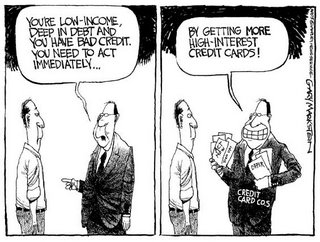
\includegraphics{cartoon.jpg}
\end{figure}

\newpage
\tableofcontents
\newpage

\section{Unit 1: Fundamental Concepts}
\subsection{Section 1: Economics}
In general terms, economics is defined as the study of how we can best increase
a nation's standard of living and citizens' happiness with the resources that we
have available to us.\\[2mm]
Standards of living include:
\begin{itemize}
    \item cars
    \item houses
    \item leisure time
    \item access to health care
    \item cleaner air
\end{itemize}

\subsubsection{Marginal Benefit \& Marginal Cost}
Marginal benefit and marginal cost can be though of as a positive cause-and-effect
in a business environment, with the benefit being the effect and cost being the
cause. When your marginal benefit is greater the marginal cost, the more likely
a positive investment is at play. For example, you may buy an expensive car for
your long commute, but it has the best MPG in the current car market and is 
heavily reliable (marginal benefit)--potentially outweighing the initial cost
(marginal cost).

\subsubsection{Difference between Macro- \& Micro- economics}
Macroeconomics focuses on the wider concepts that play a role on the entire
economy. Components of this include:
\begin{itemize}
    \item national unemployment rate
    \item inflation rate
    \item interest rate
    \item federal government budgets \& fiscal policies
    \item economic growth
    \item Federal Reserve System \& monetary policy
    \item foreign exchange rates
    \item balance of payments
\end{itemize}
Microeconomics deals with the smaller concepts of an economy such as:
\begin{itemize}
    \item supply and demand of individual goods and services
    \item price elasticity (sensitivity) of goods and services in demand
    \item production
    \item cost functions
    \item business behavior and profit maximization
    \item income inequality \& distribution
    \item effects of protectionism (tariffs, quotas, trade restrictions, etc.)
\end{itemize}
If macroeconomics is studying a forest, microeconomics is studying the
individual trees.

\subsection{Section 2: The Production Possibilities Curve}
\subsubsection{Production Choices}
Production choices are the idea that if you have limited resources to produces
various products, you want to optimize the resources at hand so that you can make
the most of the available resources, not under-use, and not over-promise a production
value that is not achievable.

\subsubsection{Points on the Curve and Trade-Offs}
In a given graph, any values that lie on the curve means that the operating cost
of the products are being used as efficiently as possible. The idea is that the
output cannot increase if it is limited by a constant resource and technology.
Scarcity talks about the limited resources at hand--which directly correlates
with the Production Possibility Curve. If a value lands on the curve, increasing
the production of one good/category will be at the expense of other goods/categories.
Points E, C, B, A, and D depicted in figure \ref{fig:GnR1} represents the most
optimized products that can be produced with resources at hand. It also shows
varying priorities for both Guns and Roses productions.

Any points that fall inside the curve (to the left of the curve, i.e point G in
figure \ref{fig:GnR1}) shows an inefficient use of resources to produce products.
Some reasons for this could be using fewer than the available resources
(unemployment), or using all resources but inefficiently (underemployment).

Points that fall outside the curve (to the right of the curve, i.e point G in
figure \ref{fig:GnR1}) shows a combination that cannot be achieved with the
available resources. This value does not mean point F will never be achievable--
the economy may grow and F may fall on or inside the Possibility curve, but at
the current analysis of the economy, it will not be possible.
Increases in technology and/or resources can help contribute to the growth of
the Production Probability Curve, which can help reach point F in the future.

\begin{figure}
    \centering
    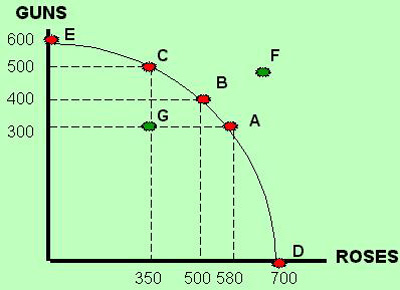
\includegraphics[width=7.5cm, height=5cm]{Production_Possibility_Curve.jpg}
    \caption{Example of a Possibility Curve of Guns and Roses production.}
    \label{fig:GnR1}
\end{figure}

\subsection{Section 3: Economic Growth}
Economic growth occurs when the economy realizes greater production levels.
Essentially, when either the number of resources increase, or the way we use
resources becomes more efficient, is the only time the curve can shift outwards.
In short, economic growth is made possible by advances in technology and/or
increase in resources.

\begin{figure}
    \centering
    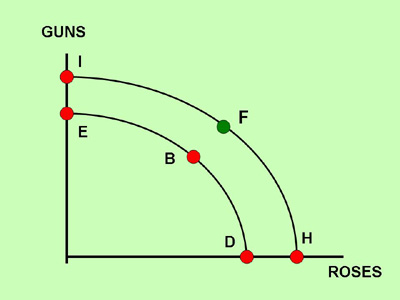
\includegraphics[width=7.5cm, height=5cm]{economic_growth_graph.jpg}
    \caption{Example of how economic growth now reaches point F.}
    \label{fig:GnR2}
\end{figure}

\subsubsection{Increase in Capital Goods}
If a country is producing at full employment, more capital goods can be produced
only inf the country produces fewer consumption goods. A few ways governments
can encourage more production of capital goods can be through tax breaks for the
production of capital goods, or increasing taxes on the production/sale of
non-capital (consumption) goods.

\subsubsection{Advances in Technology}
Advancements in technology that contribute to economic growth are usually due to
entrepreneurs who have incentives to produce more efficiently and lower their
costs. When this model is successful, this usually drives the entrepreneur to 
continue to improve their models to become more efficient with both the work/effort
needed, and the money saved. Governments that allow entrepreneurs to keep most of
their profits and tax them less has been shown to produce greater rates of
technological growth. In addition to new technology, the more human technological
advancements made (greater education, training, skills, etc), the higher the 
production probability curve also grows.

\subsubsection{Economic Growth and Economic Systems}
There are various factors that can lead a country to economic growth and downfalls.
For example, in a capitalist country, having a government that supports just 
reward systems (taxes and regulations that reward work and entrepreneurship), 
just legal system, infrastructure, national security, and protection of individual
property rights can all lead to great economic growth. Also, political incentives
can also lead to economic growth. For example, India's switch to international 
trade in the 90's has led to greater opportunities, and the same for China in
the 80's when they adopted the free market elements.

Countries that practice communistic or command economy policies have seen 
significantly less economic growth due to the sheer control the government has
over resources and entrepreneurial entrepreneurial incentives.

In third world countries, instability with governments, corruption, civil strife,
national security, and uncertainty make is extremely difficult to have a 
steady, growing economy.

\subsubsection{Conditions for Economic Growth}
Countries with the highest per-capita earnings are characterized by all or most
of the following:

\begin{enumerate}
    \item \textbf{Strong private property rights.}

        If a country does not do its best to protect the property rights of its
        citizens, then the incentive to work hard in an economic state begins
        to dwindle. If a country allows the protection of private property to
        individuals, then incentive to work hard increases, since the properties
        (land, equipment, commodities, etc) is protected and belongs to the
        individual who earned it.

    \item \textbf{Free markets, free international trade, and a stable price level.}

        Free markets are markets in which prices of goods and services, wages, 
        rents, interest rates, and foreign exchange rates are determined by the
        interaction of private sector demand and supply.

        In order for free international trade, countries need to avoid protectionism
        (tariffs, quotas, etc.)

        Stable price level is achieved when there is little to no fluctuation
        in the country's average price level. This can be achieved by a country's
        monetary agency keeping its money supply restricted or constant.


    \item \textbf{Essential government regulations and reasonable levels of
        taxation.}

        Balanced rule, regulations, and taxes must be enforced by governments in
        order for governments to provide essential functions. If there is too 
        high of a tax, businesses and individuals will be less incentivized to
        work, while excessive regulations can lead to time consuming and 
        expensive business operations. If there are high taxes and excessive
        regulations, this discourages business start-ups, make businesses fail,
        or businesses may move abroad to avoid high taxes/regulations.

    \item \textbf{Little corruption.}

        If a governments/private groups initiates force by taking away citizen's
        businesses'/private property, it does not give any incentive for individuals
        to create/continue/maintain business with that government.
\end{enumerate}

The only cause of long-term economic growth and outward shifts in the production
possibility curve  are \emph{increases in resources and advances in technology}.
More and better resources allow businesses to produce more efficiently and 
effectively, lower costs, increase real incomes and increase purchasing consumers'
power. Increasing a nation's money supply or increased government spending 
\emph{may} help in the short-run, but has economic disadvantages in the long-run.
When wages are increased, that only means that the price of goods and services will
increase. There is no profit gain for businesses, and there is no money-saved
from consumers. The only thing that has changed is the \emph{nominal} prices of
wages, goods and services. The only way to increase real profits is to increase
productivity. This also lowers costs and decreases prices, which allows increases
in real profits and real demand.

\subsection{The Circular Flow}
The way how a basic economy works is that businesses offer goods, and households
pay businesses for those goods. Households also offer services to the businesses,
and in return, businesses pays the households for their services. Government also
plays a role, since they offer neutral services to both parties (households and
businesses). Since they offer services to both parties, the parties must also 
contribute to the government for those services (in the form of taxes).

When you bring in foreign markets into account, the same principals apply for
businesses, households, and governments.

Figure \ref{ref:circular_flow} is an illustration of the circular flow of a 
basic economy.
\begin{figure}[h]
    \centering
    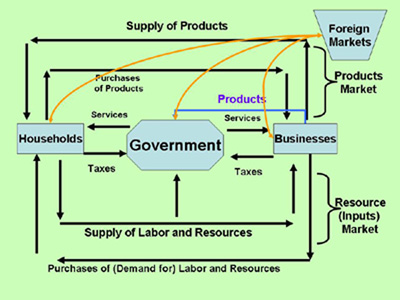
\includegraphics[width=7.5cm, height=5.0cm]{circular_flow.jpg}
    \caption{Graphical representation of how the circular flow works with 
    businesses, households, governments, and foreign markets.}
    \label{ref:circular_flow}
\end{figure}

\subsection{Economic Systems}
There are three different types of economic systems:
\begin{itemize}
    \item \textbf{Laissez-faire economy}
        represents a pure capitalist system (also called a price system). In this
        economy, the supply and demand behavior of businesses and households 
        determine the price of goods and services and factors of production. The
        government plays a very limited role and only provides the most essential
        functions such as a legal system, protecting individuals/property rights,
        and providing infrastructure and certain public goods.

    \item \textbf{Command economy}
        is a communist system where a country's government determines the prices
        of goods and services and factors of production. The country/government
        controls all of the country's economic decisions.

    \item \textbf{Mixed economy}
        is a mix between a command and laissez-faire economy. The exact mix of
        the two is dependent on the government involvement. Most industrialized
        countries follow this type of economic system.

\end{itemize}

\subsection{Important Concepts and Definitions}
Some definitions and concepts that will be used throughout these notes.

\subsubsection{Nominal and Real Values}
Nominal value (nominal wages, nominal interest rates, nominal Gross Domestic
Product, GDP) is the price of the actual dollar value which was recorded during
the transaction. This can be the price that shows up on a contract, receipt, etc.
You can think of this as the original monetary price of an invoice. Real value
is the monetary value that is reflective of the current market. For example,
lets say you bought a house 10 years ago for \$50,000, but its current market
value is \$100,000. The nominal value of the house is \$50,000, while the actual
value is \$100,000.

\subsubsection{Positive and Normative Economic Statements}
Positive economic statements are facts, or statements which can be proven. 
Positive statements does not have to be a true statement; the statement can be
proven false. It just needs to be provable. Examples of positive economic 
statements are:
\begin{itemize}
    \item The federal government experienced a budget surplus this past year
        (this is a false positive statement, but, by definition, a positive
        economic statement).

    \item When the value of the dollar falls, Japanese products imported into
        the United States become more expensive (this is a true positive statement).

    \item Legalizing drugs will reduce the drug profits that illegal drug dealers
        make (this is a true positive statement).

    \item The United States does not have a federally mandated minimum wage
        (this is a false positive statement).
\end{itemize}

A normative economic statement cannot be proven; they are opinions or value 
judgements. Examples of normative economic statements are:
\begin{itemize}
    \item The government should raise taxes and lower government spending to
        reduce the budget deficit.

    \item We need to try to lower the value of the dollar in order to discourage
        the imports of Japanese goods into this country.

    \item Our government should legalize the use of drugs in this country.

    \item The federal minimum wage should be at least \$15.00.
\end{itemize}

\subsubsection{Ceteris Paribus}
Latin for "if no other things in the economy change". When college tuition rises,
student enrollment will decrease, ceteris paribus. But if the parents' real income
increased as well, then student enrollment may increase, despite the tuition
increase. Therefore, the ceteris paribus condition is violated.

\subsubsection{Fallacy of Composition}
If you say what is good for one thing is \emph{necessarily} good for the entire
group, then you are subject to fallacy of composition. If a college has a
shortage of parking spots, your intuition is to tell students to arrive early.
But if every student comes early, there will still be a parking shortage issue.

\subsubsection{Broken Window Fallacy}
The idea that destruction stimulates the economy, therefore destruction creates
employment. This is not true. If you break a window, and hire a glazier to fix
it at the cost of \$500, the you have provided employment to the glazier. However,
if you did not break the window, you would have kept the \$500, and afterwards
you could buy a watch (which also increases employment). If you break the window,
you are gaining the employment of the glazier, but losing the employment of the
tailor. If you don't break the window, you will 1) keep the window, 2) keep the
\$500. 3) employ the tailor. Keeping the window is an important factor, since it
was already working, therefore there was no need to mindlessly destroy it in
order to hire a glazier. In general, destruction is not a good thing
microeconomicailly.

\subsubsection{Fallacy of Cause and Effect}
Basic idea of cause and effect; just because one action is immediately followed
by another action, does not mean action a caused action b to occur.

\subsection{Economics and Critical Thinking}
When looking at economic statements, scenarios, and analyses, you have to pay
attention and think about these six guidelines:
\begin{compactenum}
    \item \textbf{Question the source.}
        
        Study the background of the person making the statement to determine
        biases.
    \item \textbf{Question the assumptions.}

        Make sure you are not drawing conclusions too fast before thinking of 
        other factors that might come into play.
    \item \textbf{Question how the variables are defined.}
        
        The defining of variables is extremely important. If you are vague with
        the variables in your assumption, then you will have poor results, or
        the results you did not intend on happening. You can also be fooled by
        others' poor variable definitions, potentially swaying you and causing
        a sort of false-results. Garbage-in, garbage-out.
    \item \textbf{Question the validity of the statement.}

        Make sure the statements concluded do not fall into the fallacies, like
        the fallacy of cause and effect, and fallacy of composition (broken window
        fallacy).
    \item \textbf{Question the statistics.}

        Statistics can be meddled with, especially when you are vague with
        defining variables in your initial question.
    \item \textbf{Think like an economist.}
        
        Think practical in the sense of the real world and economics. Yes, maybe
        one solution passes the above five checks, but is it reasonable in the
        real world (outside of the math and conditions)?
\end{compactenum}

\section{Unit 2: Supply and Demand}

\subsection{The Law of Demand}
The law of demand states that buyers of a good will purchase more of the good
if its price is lower, and vice versa. This assumes that no other economic changes
take place. This law assumes ceteris paribus--no other changes take place.

\subsubsection{Substitution and Income Effects}
The substitution effect states that as the price of a product decreases, it
becomes cheaper than competing products (assuming the competing product does not
decrease in price). Consumers will substitute the cheaper product for the more
expensive product.

The income effect states that as the price of a product decreases, buyers will
have more income available to purchase more products, and vice versa. The buyer
will more likely buy more of the product that became cheaper, since they have
more expense to use on said product.

\subsection{The Demand Curve}
When graphing a demand curve, we look at two variables, product (P) and the
quantity (Q) of the product purchased during a certain time period. The demand
curve always slopes downwards. Figure \ref{fig:demand_curve} the demand curve.
\begin{figure}
    \centering
    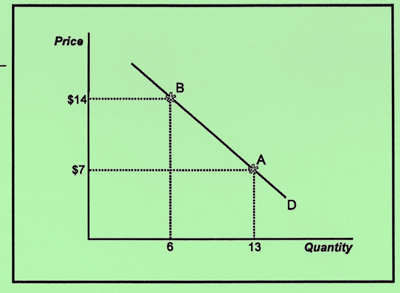
\includegraphics[height=5.5cm, width=6cm]{demand_curve.jpg}
    \caption{Graph of demand curve.}
    \label{fig:demand_curve}
\end{figure}

Market demand is the total demand for a product by all customers. Total demand
is the sum of all \emph{individual} buyers' demand.

A demand schedule and a corresponding demand curve represents the buyer's 
\emph{willingness} and \emph{ability} to purchase the product. For demand to
exist, a buyer must \emph{desire} and be \emph{able} to afford it.

Usually, a buyer's willingness to purchase a product depends on the value the 
buyer expects to receive from purchasing the product. This is called the
\textbf{utility}.

When a buyer purchases additional products, this is called the
\textbf{marginal utility}. Typically, a buyer's marginal utility decreases as 
the person consumes more of a product.

\textbf{util} is the imaginary measure of satisfaction. Since satisfaction differs
for different people and products, there is no real measurement. It is used
for comparison purposes. Utils is the measurement of utility.

Usually, more valuable items come with more utility (lets say, a car). If you do
not own a car, the first car you get will have high utility. But if you wanted
to buy a second car, the second car does not have nearly as high of a utility as
the first car did. This is called the \textbf{law of diminishing marginal utility}.

In other words, the more of a product you have, the less satisfaction you receive
from buying additional products. This does not apply for every product. Beer,
for example, usually does not follow this law (since the more you drink, the more
you will typically want).

\subsection{The Law of Supply}

\subsubsection{Price and Quantity Changes}
When ceteris paribus, product suppliers offer more of a product at a higher than
at lower prices. If a product price is high, then the supplier can make a greater
profit by selling more (assuming the price of production is constant and there
is a demand for the good).

\subsubsection{Income and Substitution Effects}
Income effect is when a business is able to sell a product for a higher price
and still sell approximately the same amount.

The substitute effect is when a supplier notices the market price of product A
increasing, ceteris paribus, producing product B will be less attractive to the
supplier. The supplier will want to produce more of product A since they can
make a better profit out of it compared to producing product B.

\subsection{The Supply Curve}
The supply curves has an upwards slope. At higher prices, firms are willing and
able to sell more than at lower prices. There is a direct relationship between
price and quantity supplied. Figure \ref{fig:supply_curve} shows the supply curve.
\begin{figure}[h]
    \centering
    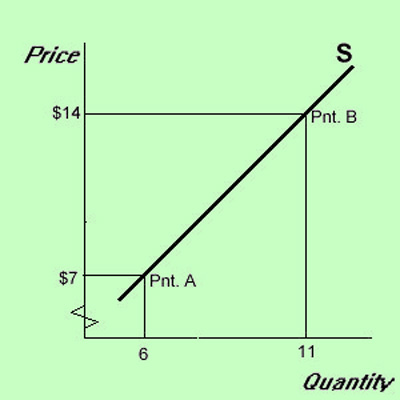
\includegraphics[height=5.5cm, width=6cm]{supply_demand_curve.jpg}
    \caption{Graph of supply curve.}
    \label{fig:supply_curve}
\end{figure}

The same principals of the demand curve applies to the supply curve.

\subsection{Equilibrium Price and Quantity}
\subsubsection{Market Price and Quantity}
When you put the supply and demand curve together, you will obtain a graph with
an intersecting point. This intersecting point is the equilibrium of what
suppliers want to price their product quantities at, and what buyers are willing
to buy quantity at certain prices. If a seller wants to sell their product 
for an extremely high price, buyers will only buy small quantities when sellers
actually want to sell a lot more. To compromise, they will lower the price. Vice
versa with buyers. Figure \ref{fig:equilibrium} an example of the equilibrium graph.
\begin{figure}
    \centering
    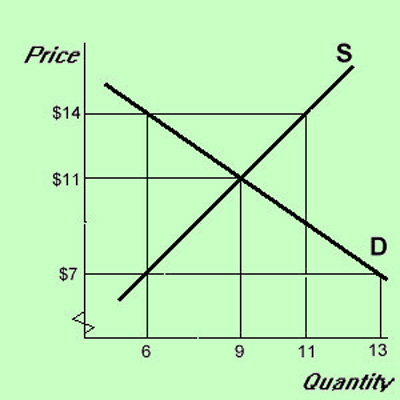
\includegraphics[height=5.5cm, width=6.0cm]{equilibrium.jpg}
    \caption{Graph of how supply and demand curves combined will create an 
    equilibrium.}
    \label{fig:equilibrium}
\end{figure}

An example of lower-limits (price floor) to the supply-demand equilibrium is
rent control. Rent control is placed below the equilibrium, so that more people
can afford housing, but doing so, landlords are less incentivized to create
those living spaces since they will not be making profits.

An example of upper-limits (price ceiling) is minimum wage. Minimum wage is set
above the equilibrium. This means that there is more incentive for workers to
want to get a job (because they will be paid more), but companies will not want
to pay this since they will lose profits. There will be less demand for
companies to hire vs the high supply of willing workers.

\subsection{Demand Determinants}
Demand curve can shift from left to right, and they are determined by these
factors;
\begin{enumerate}
   \item \textbf{A change in buyers' real income or wealth.}
       
       Usually, a normal product increases if the buyers experiences an increase
       in real incomes or wealth. However, when this happens, some products may
       experience a decrease in demand. For example, someone who could only afford
       pasta can now afford steak. Steak will become the normal product as the 
       buyer will no longer purchase pasta as much as steak since they experienced 
       the increase of real income/wealth.
        
   \item \textbf{Buyers' tastes and preferences.}

       Self explanatory, the more popular an item is, the more buyers will want
       it. Also, this will leave unpopular items to be sold less, therefore lose
       value.

   \item \textbf{The prices of related products or services.}

        A buyer always purchases product A. All of a sudden, product B is cheaper
        than product A. The buyer will instead start to purchase product B since
        it is cheaper, lowering the demand for product A, and increasing the demand
        for product B.

   \item \textbf{Buyers' expectations of the product's future price or
    availability, or their future income or wealth.}

        If buyers assume increased incomes, or product value (they believe there
        will be a shortage of toilet paper, more expensive gas prices, etc.), the
        demand will rise in the short-term (stock up on toilet paper, fill up the
        gas tanks). This will also increase the costs of those items since the
        demand also rises (in the short-term).

    \item \textbf{The number of buyers (population).}

        The more of a population, the more the demand will be. If there is a rise
        of newborn babies, there will be higher demand for baby products.

\end{enumerate}

\subsection{Change in Demand on Equilibrium Price and\\ Quantity}
When the demand curve shifts to the right, demands increases. The market price
increases, and so does the equilibrium quantity (in the short-run).

When the demand curve shifts to the left, equilibrium price and quantity decreases
(in the short-run).

\subsection{Supply Determinants}
Supply curve can shift from left to right, and they are determined by these
factors:

\begin{enumerate}
    \item \textbf{Advance in technology.}

        Advancements in technology will lower the cost of producing it, which
        increases profit. Also creates incentive to increase supply.

    \item \textbf{Change in the price of an input used to make the product.}
        
        When price of input (labor, raw materials, machinery, land) decreases,
        business makes more profit per product and is willing and able to
        increase the supply of the product (and vice versa).

    \item \textbf{Change in taxes, subsidies, or regulations.}

        Taxing or more regulations on manufacturing of a product lowers the 
        supply, because cost of producing supply increases. A subsidy (government
        grant) to a business or individual can increase the supply.

    \item \textbf{Number of suppliers.}

        When there are more competitors of a product, there will be more demand
        (and vice versa). Sometimes, government agencies can limit the amount of
        suppliers (licenses, permits, diplomas, etc) which safeguards the consumers
        to ensure they receive quality, but also limits the amount of suppliers.
\end{enumerate}

\subsection{Change in Supply on Equilibrium Price and Quantity}
An increase in supply will show the line going rightward (or downward), while
a decrease in supply will show the line going leftward (or upward).

Figure \ref{fig:supply_shift} shows an example of what this looks like.
\begin{figure}[h]
    \centering
    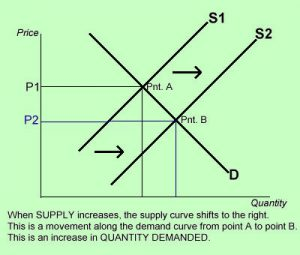
\includegraphics[height=5.5cm, width=7.0cm]{supply_shift.jpg}
    \caption{Plot of supply shift.}
    \label{fig:supply_shift}
\end{figure}

\subsection{The Effect of Change in Both Demand and Supply on Equilibrium Price
and Quantity}
When talking about short and long term changes, short term is in a time span of
several months, while long term is over a year or longer. \emph{Equilibrium
price} represents the market price (price you find at the grocery store).
When talking about the \emph{equilibrium} quantity, it represents the quantity
or amount of a certain product being bought and sold in a store.

A simple way to know when supply and demand affect price and quantity
increases/decreases is by memorizing the four conditions:
\begin{description}
\item When \textbf{demand} \emph{increases} $\Longrightarrow$ \textbf{Price}
    \emph{increases} and \textbf{quantity} \emph{increases}
\item When \textbf{demand} \emph{decreases} $\Longrightarrow$ \textbf{Price}
    \emph{decreases} and \textbf{quantity} \emph{decreases}
\item When \textbf{supply} \emph{increases} $\Longrightarrow$ \textbf{Price}
    \emph{decreases} and \textbf{quantity} \emph{increases}
\item When \textbf{supply} \emph{decreases} $\Longrightarrow$ \textbf{Price}
    \emph{increases} and \textbf{quantity} \emph{decreases}
\end{description}

\subsection{Demand vs Quantity Demanded and Supply vs Quantity Supplied}
\subsubsection{The Difference between Demand and Quantity Demand}
If the market price of a product decreases, then the \emph{quantity demand} increases,
and vice versa. For example, when the price of strawberries decreases (while 
in season), more customers will purchase strawberries. Figure \ref{fig:quant_dem}
how the quantity demand has changed by a movement \emph{along} the demand curve.
\begin{figure}[h]
    \centering
    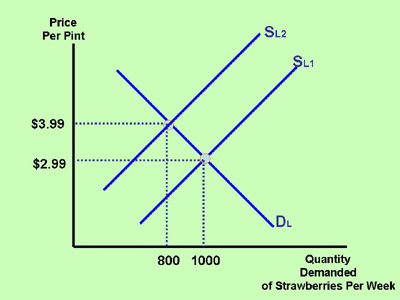
\includegraphics[height=5.5cm, width=7cm]{quantity_demand.jpg}
    \caption{Change in quantity demand.}
    \label{fig:quant_dem}
\end{figure}

When one or more of the five demand determinants (see section 2.6) changes, then
\emph{demand} changes. For example, when buyers' income increase, the \emph{demand}
(not the quantity demanded) for a normal product increases. Or when the price of
a substitute product decreases, then the demand for the product in question 
decreases. Or when the number of buyers increases, the demand increases, and the
price of the product increases. An increase in demand is shown by a \emph{rightward
shift} in the demand curve. See Figure \ref{fig:demand_shift} as a reference.
In the graph, demand increases as D1 shifts to D2. \emph{Quantity supplied} also
increases as the equilibrium points shift along the supply curve from point A
to point B.
\begin{figure}[h]
    \centering
    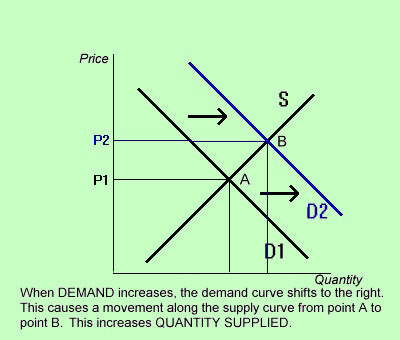
\includegraphics[height=5.5cm, width=7cm]{demand_shift.jpg}
    \caption{Graph depicts the change of demand going rightwards.}
    \label{fig:demand_shift}
\end{figure}

\subsubsection{The Difference between Supply and Quantity Supplied}
If the market price of a product increases, then the \emph{quantity supplied}
increases, and vice versa. For example, when housing prices increase, more
people will want to sell their house. See Figure \ref{fig:quant_supp} below as a
reference of how quantity supplied affects supply.
\begin{figure}[ht]
    \center
    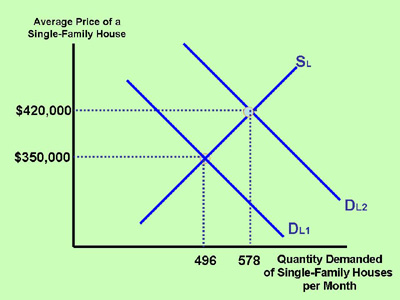
\includegraphics[height=5.5cm, width=7cm]{quantity_supplied.jpg}
    \caption{The graph depicts the number of goods increasing as price increases
    as well.}
    \label{fig:quant_supp}
\end{figure}

When one or more of the four supply determinants (See 2.8) changes, then \emph{
supply} changes. For example, when technology advances, or the cost of production
decreases, \emph{supply} increases. See Figure \ref{fig:supply_quant_shift} below 
as a reference.
\begin{figure}[ht]
    \center
    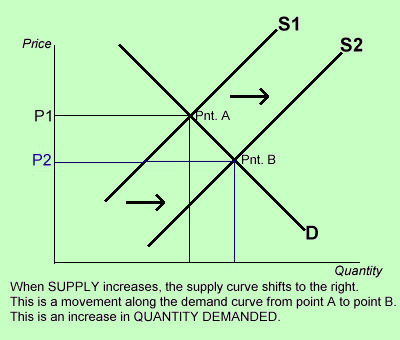
\includegraphics[height=4.5cm, width=6cm]{supply_quant_shift.jpg}
    \caption{As supply increases from as S1 shifts to S2, quantity increases as
    the equilibrium points shift along the demand curve from point A to point B.}
    \label{fig:supply_quant_shift}
\end{figure}

\subsection{Consumer Surplus and Producer Surplus}
Producer surplus happens when the price changed by businesses is higher than the
equilibrium (businesses are producing more than what consumers are buying).
Consumer surplus happens when businesses charge at the equilibrium price, but
consumers are willing to pay above the equilibrium price since they value the 
item a lot.
\subsubsection{Consumer Surplus}
The difference between how much consumers value a product and how much they
actually pay for it at the equilibrium price is called \emph{consumer surplus}.
Figure \ref{fig:consumer_suprlus} below shows the area which consumer surplus lies.
\begin{figure}[ht]
    \center
    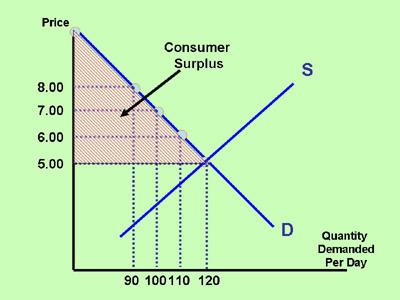
\includegraphics[height=4.5cm, width=6cm]{consumer_surplus.jpg}
    \caption{Red area indicates where consumer surplus lies.}
    \label{fig:consumer_suprlus}
\end{figure}

\subsubsection{Producer Surplus}
Producer surplus is similar to consumer surplus, but it measures the benefits
of a trade for producers. \emph{Producer surplus} is the difference between the
minimum price at which producers would have been willing to produce the product
and how much they are actually receiving at equilibrium.
Figure \ref{fig:producer_surplus} below shows the area which producer surplus lies.
\begin{figure}[ht]
    \center
    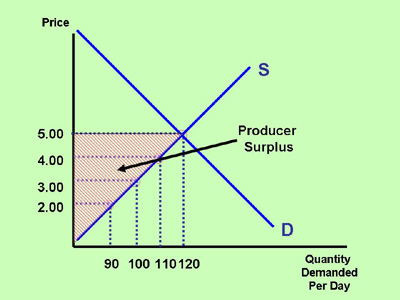
\includegraphics[height=4.5cm, width=6cm]{producer_surplus.jpg}
    \caption{Red area indicates where producer surplus lies.}
    \label{fig:producer_surplus}
\end{figure}

\section{Unit 3: Elasticity}
Elasticity is how much the price of a good fluctuates depending on decrease in
demand. If the price of a product increases and the amount demanded decreases
by a lot, then the product is \emph{elastic}. If it decreases by a little, or
not at all, then the product is \emph{inelastic}.

\subsection{Demand Curves and Elasticity}
\subsubsection{Price Elasticity of Demand}
\emph{Price elasticity of demand} measures the responsiveness of buyers to a
price change. In other words, it measures the relationship between the percentage
change in the amount of purchased and the percentage change in the price.

\subsubsection{Derivation of a Demand Curve}
The type of data that economist use to estimate the shape and location of a
product's demand curve are:
\begin{enumerate}
    \item \textbf{Historical Data}

        Price and quantity data show how consumers have responded to past changes
        in the price and quantity demand of the product. Price and quantity demand
        changes must be looked at in isolation of other variables. \textbf{It is
        important to estimate the price and quantity demand changes assuming
        other variables remain constant (ceteris paribus).}
    \item \textbf{Surveys}

        If you ask customers their input on how they would respond to a future
        change in the price of the product, you may not get accurate data, but
        it will allow economist to estimate the location and slope of a demand
        curve. When you know the location and slope of a product's demand curve,
        you can determine its \emph{price elasticity of demand}.
\end{enumerate}

\subsubsection{Formula for Price Elasticity of Demand}
The law of demand states that as the price of a product decreases, quantity
demand increases, and vice-versa. Elasticity measures \textbf{how much} less
people buy of that product when the prices rises, and vice-versa. Price 
elasticity of demand is determine by looking at the ratio of:
\begin{description}
    \item \textbf{e = The percentage change in quantity demand divided by the
        percentage change in the price of the product.}
    \item or
    \item \textbf{e = $\frac{\text{\% change in Q}}{\text{\% change in P}}$ }
        
        \item where:

        \begin{enumerate}
            \item \textbf{The \% change in Q = $\frac{\text{change in quantity
                demanded}}{\text{average of the two quantities in demand}}$}
            \item \textbf{The \% change in P = $\frac{\text{change in price}}
            {\text{average of the two prices}}$}
        \end{enumerate}

    \item The formula above is called the "arc" formula. It is the most accurate
        and most commonly used in economics.
\end{description}

\subsection{Elasticity and the Slope of the Demand Curve}
\subsubsection{Demand Curves and Elasticity}
Elasticity affects the slope of a product's demand curve. A greater slope, the
steeper the demand curve is and a less-elastic product. Figure \ref{fig:dem_cur_ela}
below is a visualization of what each line means in terms of elasticity.
\begin{figure}[h]
    \centering
    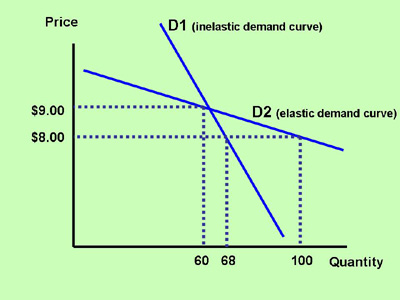
\includegraphics[height=4.5cm, width=6cm]{demand_curve_elasticity.jpg}
    \caption{In line D1, you can see when the cost goes down from \$9 to \$8,
    the demand only slightly increases (from 60 to 68), while the line D2--when
    the cost goes down from \$9 to \$8, the demand increases a lot more (from
    60 to 100). These are the effects of slope and elasticity.}
    \label{fig:dem_cur_ela}
\end{figure}

\subsubsection{Perfect Elasticity and Perfect Inelasticity}
\emph{Perfect elasticity} is when a product can only be set at one price. If the price
change then the quantity demand changes to zero.

\emph{Perfect inelasticity} is when a product can only be bought at one quantity
size, no matter the price of the product.

Figure \ref{fig:perf_elast} below is a graph of both perfect elasticity and
perfect inelasticity.
\begin{figure}[ht]
    \centering
    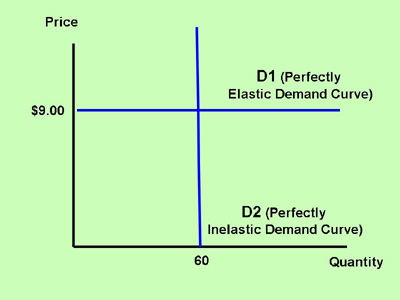
\includegraphics[height=4.5cm, width=6cm]{perfect_elasticity.jpg}
    \caption{Example of both perfect elasticity and inelasticity}
    \label{fig:perf_elast}
\end{figure}

\subsection{Determinants of Price Elasticity of Demand}
\subsubsection{Elasticity Determinants}
Some products are elastic (buyers are price sensitive), and some products are 
inelastic (buyers are not price sensitive). For some products (cars vs salt), 
price elasticity of demand can make a huge impact for the buyer (10\% increase 
in a car's value has more impact than 10\% increase in the value of salt.)

There are three determinants of price elasticity of demand:
\begin{enumerate}
    \item \textbf{The availability of close substitutes}
        
        If there are a lot of close substitutes available, then people will
        react strongly to price increases. Price elasticity of demand is high.

    \item \textbf{The importance of the product's cost in one's budget}

        If a product is inexpensive to a consumer's budget, then increases in
        price will not matter that much. Mostly everyone has a budget for salt,
        so a 10\% increase will not impact the consumer as much. But if the
        consumer wants to purchase a car (clearly, a car is not on a consumer's 
        usual budget), a 10\% will matter a lot more.

    \item \textbf{The period of time under consideration}

        Price elasticity of demand is greater the longer it takes for a product
        to increase its price. This gives consumers more time to adjust to
        increasing prices whereas if it is an immediate jump in price, it will
        cause more issues for consumers.

        For example, if the price of gas increases immediately, car owners may
        not decrease the mileage they drive in the first week, but after a
        couple of years, they may buy a more fuel-efficient car, move closer to
        school/work, etc.
\end{enumerate}

\subsubsection{Elasticity and the Effect of a Tax Change on the Price of the
Product}

How much equilibrium price of a product will increase with taxes depends on the
product's elasticity. The demand curve slope can help determine the price of the
products after a new tax is imposed. Figure \ref{fig:combined} below are two
graphs to show the difference in prices with different slopes.

\begin{figure}[ht]
    \centering
    \begin{subfigure}{0.41\textwidth}
        \centering
        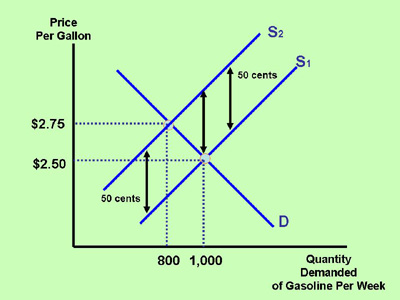
\includegraphics[width=\textwidth] {elasticity_tax_minimal.jpg}
        \caption{With higher elasticity, you will get lower price change (less
        steep slope).}
        \label{fig:left_elas}
    \end{subfigure}
    \hspace{1mm}
    \begin{subfigure}{0.42\textwidth}
        \centering
        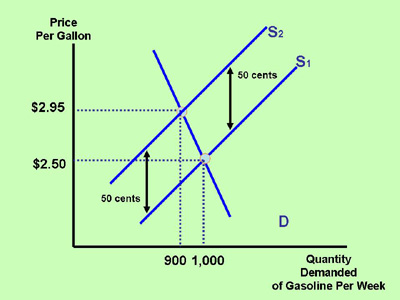
\includegraphics[width=\textwidth] {elasticity_tax_max.jpg}
        \caption{With lower elasticity, you will get a higher price change 
        (steeper slope).}
        \label{fig:right_elas}
    \end{subfigure}
    \caption{Side-by-side comparison visualizing a 50\textcent \space tax
        increase with two different elasticity slopes.}
    \label{fig:combined}
\end{figure}
In general, for less-elastic products (steeper demand curves), the burden of the
tax is mostly on the consumer. For more-elastic products, the burden of the tax
is mostly on the suppliers.

\subsection{Elasticity and Total Revenue}
\subsubsection{Definition of Elastic, Inelastic, and Unit Elastic Demand}
By definition:
\begin{description}
    \item \textbf{A product is elastic when its elasticity is greater than 1.}

        When a product is elastic and its price changes, the percentage change
        in quantity demanded is greater than the percentage change in the price.

        As an example, if buyers purchase 20\% fewer products as a result of a
        10\% price increase, then the product is elastic.
    \item \textbf{A product is inelastic when its elasticity is less than 1.}

        The numerator (percentage change in quantity demanded) of the elasticity
        formula is less than the denominator (percentage change in price).

        As an example, if buyers purchase 6\% fewer products as a result of a 
        15\% increase, then the product is inelastic.
    \item \textbf{A product is unit elastic when its elasticity is equal to 1.}

        If a product's price rises by 8\% and its quantity demanded decreases by
        8\%, then the product is unit elastic.
\end{description}

\subsubsection{Elasticity and Revenue}
A businesses total revenue is equal to the number of products it sells times the
price of the product, therefore:
\begin{description}
    \item \textbf{Total Revenue = Price times Quantity}
    \item or
    \item \textbf{$TR = P \times Q$}
\end{description}

If a product is \emph{elastic}, the percentage change in the quantity demanded
change is greater than the percentage change in the price. Therefore, for an
elastic product, if the price increases, the percentage change in the quantity
demanded decreases by a greater amount, and the firm's revenue will decrease,
and vice-versa.

if a product is \emph{inelastic}, the percentage change in the quantity demanded
change is smaller than the percentage change in the price. Therefore, for an 
inelastic product, if the price increases, the percentage change in the quantity 
demanded decreases by a smaller amount, and the firm's revenue will increase,
and vice-versa.

In summary:
\begin{description}
    \item When a product is elastic and its price falls, total revenue
        increases.
    \item When a product is elastic and its price rises, total revenue
        decreases.
    \item When a product is inelastic and its price rises, total revenue
        increases.
    \item When a product is inelastic and its price falls, total revenue
        decreases.
    \item When a product is unit elastic and its price changes, total revenue
        remains constant.
\end{description}

\subsection{Income Elasticity of Demand, Cross Price Elasticity of Demand, and 
Price Elasticity of Supply}
\subsubsection{Income Elasticity of Demand}
Income elasticity of Demand measures the percentage change in a buyer's purchase
of a product as a result of a percentage change in their income. Income elasticity
is:
\begin{description}
    \item $e_i = \frac{\textbf{percentage change in demand}}
                      {\textbf{percentage change in income}}$ 
    \item or
    \item $e_i = \frac{\textbf{(change in demand / average demand)}}
                      {\textbf{(change in income / average income)}}$
\end{description}

If the income elasticity demand is \emph{positive}, that means the buyer is
purchasing a normal good with their increased income.
If the income elasticity \emph{demand} is negative, that means the buyer is
purchasing an inferior good, therefore the buyer can afford more expensive
goods if they decide to purchase fewer of the inferior goods (the numbers we
used to calculate the income elasticity).

\subsubsection{Cross Price Elasticity of Demand}
Cross price elasticity of demand can measure the price change of one product's 
affect on the demand for another substitute product (i.e apples and oranges).

The formula for the cross price elasticity of demand for product A relative to
a price change in product B is:
\begin{description}
    \item $e_{cp} =
        \frac{\textbf{percentage change in the demand for product A}}
             {\textbf{percentage change in the price os subsituute prodcut B}}$
    \item or
    \item $e_{cp} = \frac{\textbf{(change in the quantities of product A /
                                    average of the quantites of product A)}}
                          {\textbf{(change in price of product B / 
                                    average of product B prices)}}$
\end{description}

\subsubsection{Price Elasticity of Supply}
Price elasticity of supply measures the percentage change in the quantity 
supplied by produces divided by the percentage change in the price of the
product.

\section{Unit 4: Business Production Behavior}
\subsection{Factors of Production}
There are three factors of production (inputs):
\begin{enumerate}
    \item \textbf{Land.}

        Land includes land and other natural, non-man-made materials, such as
        raw materials, energy sources, and trees. The payment for the use of 
        land is called "rent" in economics.

    \item \textbf{Labor.}

        Labor includes all forms of human productive effort, from blue collar 
        (manual labor) to white collar (office and management work) to 
        entrepreneurial activities (organizing resources, coming up with ideas,
        taking risks) to professional athletes and celebrities. Rewards for 
        non-entrepreneurial labor are called wages, salaries, bonuses, or 
        commissions. Entrepreneurs earn "profits".

    \item \textbf{Capital Goods.}
        
        Capital goods represent the man-made machines, equipment, buildings, 
        and other tools used to produce products. When the term "capital" is 
        used by itself, we refer money used to finance the purchase of capital
        goods. When businesses borrow money to purchase goods, they pay "interest"
        to the lenders.
\end{enumerate}

\subsubsection{Factor Prices}
Factor prices are the payments for land, labor, and capital goods. They include:
\begin{enumerate}
    \item \textbf{Wages:} Payments and rewards for (the price of)
        non-entrepreneurial labor.

    \item \textbf{Rent:} Payment and reward for the use of land.

    \item \textbf{Interest:} Payment and reward for capital (money) used to
        purchase capital goods.

    \item \textbf{Profits:} Payments and rewards for entrepreneurial
        efforts.
\end{enumerate}

\subsubsection{Factor Prices in the Free Market}
Without government involvement, prices of labor and land are determined by the
supply and demand of the factors of products provided above. If demand for land
increases (ceteris paribus), then the price of land increases, and vice-versa.
If demand for a particular type of labor increases, then the price of the labor
(wage) increases, and vice-versa. Figure \ref{fig:free_market_dia} shows the
supply and demand lines that are presented in a free market.

\begin{figure}[ht]
    \centering
    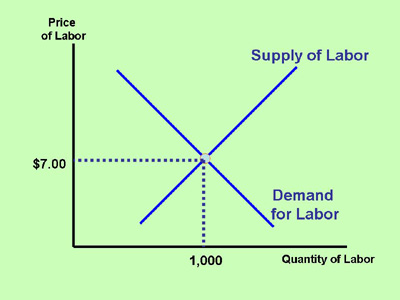
\includegraphics[height=5.5cm, width=7cm]{factors_of_free_market.jpg}
    \caption{Increase in demand for labor is illustrated by a rightwards shift
    would increase the equilibrium prince, and vice-versa.}
    \label{fig:free_market_dia}
\end{figure}

\subsubsection{Government Price-Setting}
Free market economies lead to the most economically efficient allocations of 
resources. When governments set a price above or below the free market equilibrium,
then a surplus or shortage of goods will occur. In a free market, this is avoided
since producers surplus at their highest levels (that consumers will buy). Typically,
governments have good social intentions when setting certain prices on products;
while this may help specific groups in the short-term, there will be a backfire
in economic efficiency in the long-run.

Since free markets provide more incentive to produce as efficiently as possible,
the profits may motivate businesses to increase productivity. With greater
productivity, there are more jobs, higher real wages, better products, and a
higher standard of living in the long run.

\subsection{Production Functions and the Law of Diminishing Marginal Production}
\subsubsection{Production Function}
A production function is a relationship between inputs (factors of production)
and outputs (products). Illustrates how many workers and machines it might take
to produce goods.

\subsubsection{Short Run vs Long Run}

\begin{description}
    \item \emph{Short run} is a time period during which a business cannot vary
        one or more factors of production. At least one input is fixed.

    \item \emph{long run} is a time period during which the firm has the
        flexibility to change all inputs. They can buy bigger machines, hire
        more workers, expand buildings.
\end{description}
The length of each run is dependent on the company at hand. A software company
will have a shorter length of runs vs a factors.

\subsubsection{Fixed and Variable Inputs}
\emph{Fixed inputs} remain constant in the short run, even as production 
\\decreases/increases. Examples of fixed inputs are land, heavy machinery,
buildings, and workers on long-term contracts.
\\
\emph{Variable inputs} can be varied in the short run; as in, they can 
\\increase/decrease as production increases/decreases. Examples of variable inputs
are hourly and part-time labor, office supplies, energy, and raw materials.

\subsubsection{Total, Average, and Marginal Production}
\emph{Marginal production of labor} is how much one additional worker adds to
the total production.
\\
\emph{Average production of labor} is the production per worker.
\\
\emph{Total production} is how much production of a good is created.

Below in Figure \ref{fig:car_manu} a table of a hypothetical car manufacturer's production
schedule during a short-run period of time.We assume that the firm has fixed
and variable inputs.

\begin{figure}[h]
    \centering
    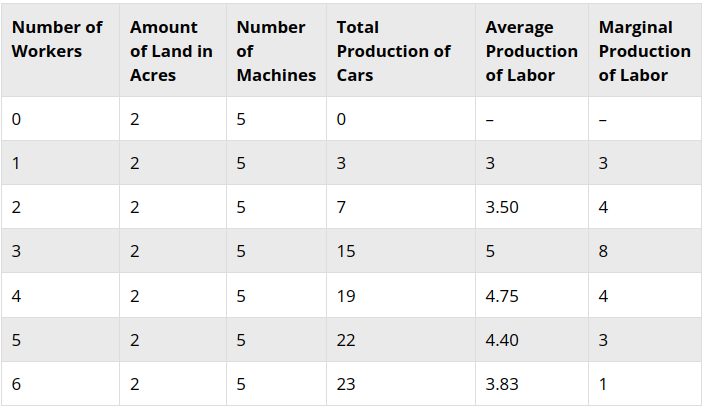
\includegraphics[width=0.76\textwidth]{car_manufact.png}
    \caption{Example of how marginal and average production of labor affect
    production levels.}
    \label{fig:car_manu}
\end{figure}

\subsubsection{Law of Diminishing Marginal Production}
The law of diminishing marginal production states that when a firm uses a variable
input, such as labor, the additional productivity of workers who are hired at a 
later stage is less than the additional productivity of workers who were hired first.

Looking at Figure \ref{fig:car_manu} above, the first three workers hired,
worker 1, 2, and 3 have a production level of 3, 4, and 8 respectivly. However,
looking at workers 4, 5, and 6, they have decreasing prodution levels of 4, 3, 
and 1. This is an example of the diminishing marginal production.

The first three workers (variable inputs) have more production because they 
have more resources to use from the land and machines (fixed inputs). They can
become more 'specialized.'

Once the firm starts to hire workers 4, 5, and 6, those workes (variable inputs)
have less access to office space, machinery, etc. (fixed inputs), therefore, 
they will have less production compared to the first three workers.

Since the diminishing marginal production occurs when there are fixed inputs,
this means the diminishing marginal prodcution law only occurs in short runs,
and are non-existent in long runs (since in long runs, every input can be changed).

In long runs, average and marginal production can decrease, but for different
reasons. A company can grow too large and bureaucratic and lose efficency. 
When this happens,the business expereineces "decreasing returns to sales" and 
"diseconomies of scale."

\subsubsection{Total, Marginal, and Average Production Graphs}
The graphs below (Figure \ref{fig:sep_prod_graphs} the three different graphs
for total production, marginal production, and average production.

\begin{figure}[ht]
    \centering
    \begin{subfigure}{0.33\textwidth}
        \centering
        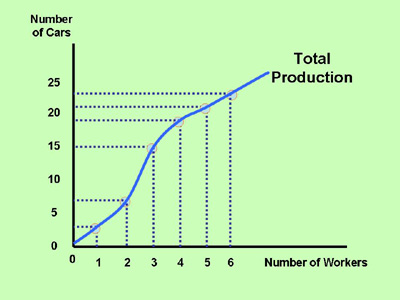
\includegraphics[width=\textwidth] {tot_prod.jpg}
        \caption{Total Production}
        \label{fig:tot_prod}
    \end{subfigure}
    \hspace{1mm}
    \begin{subfigure}{0.33\textwidth}
        \centering
        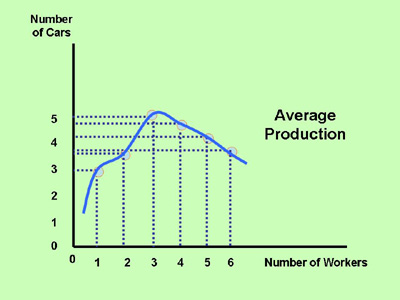
\includegraphics[width=\textwidth] {avg_prod.jpg}
        \caption{Average Production}
        \label{fig:tot_avg}
    \end{subfigure}
    \hspace{1mm}
    \begin{subfigure}{0.33\textwidth}
        \centering
        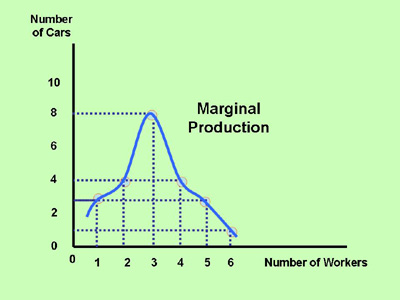
\includegraphics[width=\textwidth] {marg_prod.jpg}
        \caption{Marginal Production}
        \label{fig:tot_marg}
    \end{subfigure}
    \caption{A compilation of Total, Average, and Marginal Production Graphs.}
    \label{fig:sep_prod_graphs}
\end{figure}

In order to calculate the marginal production of labor value, you will have to
divide the change in total production by the change in the number of workers.

In Figure \ref{fig:car_manu}, to find the marginal production at a level of 3
workers, you will perform the following:
\begin{description}
    \item  $\text{Marginal Production Labor} = \frac{15 - 7}{3 - 2}$
\end{description}
Which equates to 8 (which is already given in the table, assuming the value was
missing).
\end{document}
